\chapter[Connecting Chromophore Design with Crystal Morphorology]{Connecting Chromophore Design with Crystal Morphorology}
\label{chapter: Connecting}
\section{Introduction}\label{section: Connecting_Introduction}

In Chapters \ref{chapter:NRdecay} and \ref{chapter: Inter} the \acp{PES} of a range of \ac{HC} derivatives were mapped,  in both vacuum and the crystalline form. Through the topology of the PESs and the associated energy differences between states, we determined the radiative and nonradiative relaxation channels and rationalise the observed \ac{AIE} of \ac{HC}\textbf{1} and the nonemission of \ac{HC}\textbf{5}. By elucidating the AIE mechanism of \textbf{1} and the nonemission of \textbf{5}, we isolated three design principles to increase the quantum yield of fluorescence for ESIPT chromophores in the solid state.

In this Chapter, the scope of the study is extended as the design rules established in Chapter  \ref{chapter: Inter} are applied to a new set of ESIPT systems. Into the test set we add two fluorene-substituted \ac{HC} derivatives, \ac{HC}\textbf{6} and \textbf{7}.\cite{Cheng2016}. Furthermore, and most pertinently, four completely new compounds with lasing properties are considered.  Closely related to \acp{HC} are the family of \ac{HP} derivatives.\cite{Tang2016} In contrast to \acp{HC}, and other organic fluorophores, \ac{HP} compounds contain only a single aryl group and have remarkable QEs, ranging from 0.72-0.84. This has been qualitatively attributed in experimental studies to the herringbone packing mode and molecular rigidity reducing nonradiative decay. The increased quantum yield of the \acp{HP}, with respect to the \acp{HC}, make them prime candidates to test the efficacy of our  design rules. The eleven compounds studied in this Chapter are summarised in \label{table: chalcones}. 

\begin{table}[H]
\caption[Molecular structures and their QEs ($\Phi$) in the solid state]{Molecular structures and their QEs ($\Phi$) in the solid state\cite{Cheng2015,Tang2016,Cheng2016} } 
  \label{table: chalcones}
  \begin{tabular*}{\linewidth}{@{\extracolsep{\fill}}llllllll}
  %\hline
  \multicolumn{4}{c}{
  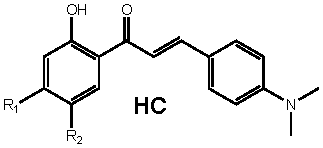
\includegraphics[height=2.15cm]{HC.pdf}}
  & 
  \multicolumn{4}{c}{
  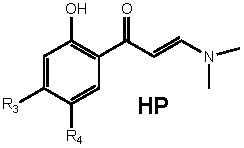
\includegraphics[height=2.15cm]{HP.pdf}}\\
  \hline
  %\multicolumn{4}{c}{\textbf{HC}}&
  %&\multicolumn{4}{c}{\textbf{HP}}\\
  & R\textsubscript{1}
  & R\textsubscript{2}
  & $\Phi$
  &
  & R\textsubscript{3}
  & R\textsubscript{4}
  & $\Phi$\\
  \hline
  \textbf{HC1} & \ce{H} & \ce{H} & 0.32
  & \textbf{HP1} & \ce{H} & \ce{H} & 0.74\\
  %\hline
  
  \textbf{HC2} & \ce{CH3} & \ce{H} & 0.25
  & \textbf{HP2} & \ce{F} & \ce{H} & 0.84\\
   % \hline
    
  \textbf{HC3} & \ce{OCH3} & \ce{CH3} & 0.26
  & \textbf{HP3} & \ce{H} & \ce{OCH3} & 0.77\\
   %  \hline
     
  \textbf{HC4} & \ce{H} & \ce{CH3} & \textless0.01
  & \textbf{HP4} & \ce{H} & \ce{F} & 0.72\\
  %\hline
  \textbf{HC5} & \ce{H} & \ce{OCH3} &\textless0.01 & & & &\\
 % \hline
  \textbf{HC6} & \ce{F} & \ce{H} &0.41 & & & &\\
 % \hline
  \textbf{HC7} & \ce{H} & \ce{F} &0.10 & & & &\\
  \hline 
  \end{tabular*}
\end{table}

Herein we investigate the factors which mediate the increased fluorescence activity for \textbf{HP} compared to \textbf{HC} systems. In Chapter \ref{chapter: Inter}, guidelines to enhance radiative decay were established for ESIPT emitters in lasing applications, based on a three step mechanism; I) localisation of excited state to one monomer, II) bias for K* decay over E*, III) an energetically inaccessible conical intersection. In the following sections each of these steps are addressed in turn to show how the \acp{HP} systems show an increased potency in each step compared to their \acp{HC} counterparts, resulting in increased fluorescence in the solid state. Particular focus will be given to \textbf{HC1}, \textbf{HC5}, and \textbf{HP1}, which will act as exemplar systems due to their differing fluorescence behaviour.

After outlining the computational methods used, the crystal structures of the eleven systems shall be analysed with particular attention paid to the dimer motifs present. Next, we examine how the dimer motifs mediate the excitonic coupling between molecular sites in the crystal and afford localisation of the excited state. An exciton hopping model based on Marcus Theory is applied to examine the different hopping rates in the enol state and examine the competition between localisation and exciton diffusion. Following this, we examine in detail the propensity for ESIPT in the \ac{HP} systems compared with their \ac{HP} counterparts. Finally, the solid state \ac{PES}  of \ac{HP}\textbf{1} is mapped, where the energy of the \ac{MECI} is shown to be prohibitively high.
%%%%%%%%%%%%%%%%%%%%% 
%%%%%%%%%%%%%%%%%%%%% 
\section{Computational Details}\label{section: Connecting_Comp}
%%%%%%%%%%%%%%%%%%%%% 
%%%%%%%%%%%%%%%%%%%%% 
Crystal structures of compounds \ac{HC}\textbf{1}-\textbf{7} and \ac{HP}\textbf{1}-\textbf{4} were obtained from the CCDC as described in references{~\citenum{Cheng2015,Cheng2016,Tang2016}}. \ac{HC}\textbf{1}-\textbf{5} and  \ac{HP}\textbf{1}-\textbf{4} were optimised in vacuum in the \szero{} and \sone{} enol and keto states at the (TD-)$\omega$B97X-D/6-311++G(d,p) level of theory. Relaxed geometry scans of the torsional rotation angle $\theta_{tor}$ in the keto \sone{} state (\Kstar) were performed for the same compounds. Proton migration scans of the ESIPT process were also performed in vacuum for \ac{HC}\textbf{1} and \ac{HP}\textbf{1}. All scans were calculated at TD-$\omega$B97X-D/6-31G(d). 

Crystal structures of all \ac{HC} and \ac{HP} compounds were optimised using Quantum Espresso in the periodic DFT framework.\cite{QE-2009} Optimisation of each unit cell was carried out with DFT-D2 (PBE) with a plane-wave cutoff of 30 Ry and ensuring Monkhorst-Pack k-point convergence in each case.

Exciton couplings \textit{J} were calculated for dimers in each optimised crystal structure. A 2x2x2 supercell was constructed for each system and a dimer was defined as any molecular pair with an interatomic distance less than or equal to the van der Waals radii of the atoms, plus a damping factor of 1.5\AA. This selection criterion has previously been used in similar applications.\cite{Campbell2017} 

To calculate solid state reorganisation energies in the adiabatic approximation ($\lambda_{A}$) for each compound we generated cluster models based on the 2x2x2 supercell, where all molecules which lay within 20{\AA} of the central chromophore were included in the cluster. Geometries were optimised in \sone{} and \szero{} states within the ONIOM protocol at $\omega$B97X-D/6-31G(d):UFF using electronic embedding. MM charges were derived automatically using the QEq method.\cite{Rappe2007} The UFF forecefield was chosen here due to the automatic charge assignment, allowing the highthroughput generation of structures and input files. In the cases of \ac{HC}\textbf{1}-\textbf{4} and \ac{HC}\textbf{6}-\textbf{7}, $\lambda_{A}$ was calculated for both enol and keto pathways. For \textbf{HC5} and \textbf{HP1}-\textbf{4}, only the $\lambda_{A}$ associated with keto relaxation was used since no \Estar{} minimum was located in the monomer QM:MM relaxation. Reorganisation energies in the normal-mode approximation ($\lambda_{NM}$) were calculated using the DUSHIN program for \textbf{HC5} and \textbf{HP1} using a reduced cluster with the 3-21G* basis set to reduce the computational cost of calculating analytic QM:MM frequencies.\cite{Reimers2001}

As the exemplar parent \ac{HP} compound, the full excited state decay mechanism of \ac{HP}\textbf{1} was established through QM:MM cluster models using density functional and multireference methods. A monomer and trimer chromophore at the centroid of the 20{\AA} cluster were optimised in the ground and excited states at (TD-)$\omega$B97X-D/6-31G(d):AMBER level of theory. The \sone/\szero{} MECI in both monomer and trimer cluster models were calculated using a modified version of the CIOpt algorithm.\cite{Levine2008} 

The MECI in the monomer cluster models was also obtained with the state-averaged complete active space self-consistent field method, employing the \szero{} and \sone{} states in the averaging. The active space consisted of 12 electrons in 11 orbitals (SA-2-CASSCF(12,11)). The 6-31G(d) basis set was using for the QM region and the AMBER forcefield was used to describe the MM region. Calculating the MECI with CASSCF:MM ensures the validity of the TD-DFT:MM-calculated MECI. The potential energy profile was refined with multistate complete active space second-order perturbation theory (MS-3-CASPT2(12,11)/6-31G(d):AMBER), incorporating the \szero{}, \sone{}, and \stwo{} states. The TD-DFT:MM geometries from the trimer models at the Franck-Condon, \sone{} minimum, and MECI were taken as the reference geometries, where the central molecule was taken for the CASPT2 calculation and the remaining two molecules of the trimer were added to the MM region.  A three state average was used due to incorporate the n$\pi^{\ast}$ \stwo{} electronic state at the Franck-Condon geometry. The orbitals chosen for the active space are shown in the Supporting Information. All density functional calculations were performed in the Gaussian 09 suite of programs.\cite{g09} CASSCF and CASPT2 calculations used OpenMolcas with the Tinker v.6.3.3 interface.\cite{Aquilante2016}

To analyse the spatial environment for the monomers at the centre of the cluster models in the each crystal, Voronoi cells partition the crystal into molecular regions. These cells define all the points in space which are closer to the reference molecule than an exterior molecule. Dividing the Voronoi cell volume by the van der Waals volume gives a molecule-independent Voronoi index $V_{i}$ for each crystal structure. To generate the Voronoi cells, a cluster of molecules was extracted from its crystalline positions. A real space grid was generated at an arbitrary resolution and at each point of this grid, the distance to each atom was calculated and scaled by the corresponding van der Waals radius. All voxels with the lowest scaled distance belonging to an atom of the central molecule were marked as belonging to the accessible of the molecule, resulting in an irregular polyhedron of finite volume. 
%%%%%%%%%%%%%%%%%\\
%%%%%%%%%%%%%%%%%
\section{Results}\label{section: Connecting_Results}
%%%%%%%%%%%%%%%%%
%%%%%%%%%%%%%%%%%
\subsection{Crystal packing motifs} \label{section: Connecting_Motifs}
\begin{figure}[H]
\centering
  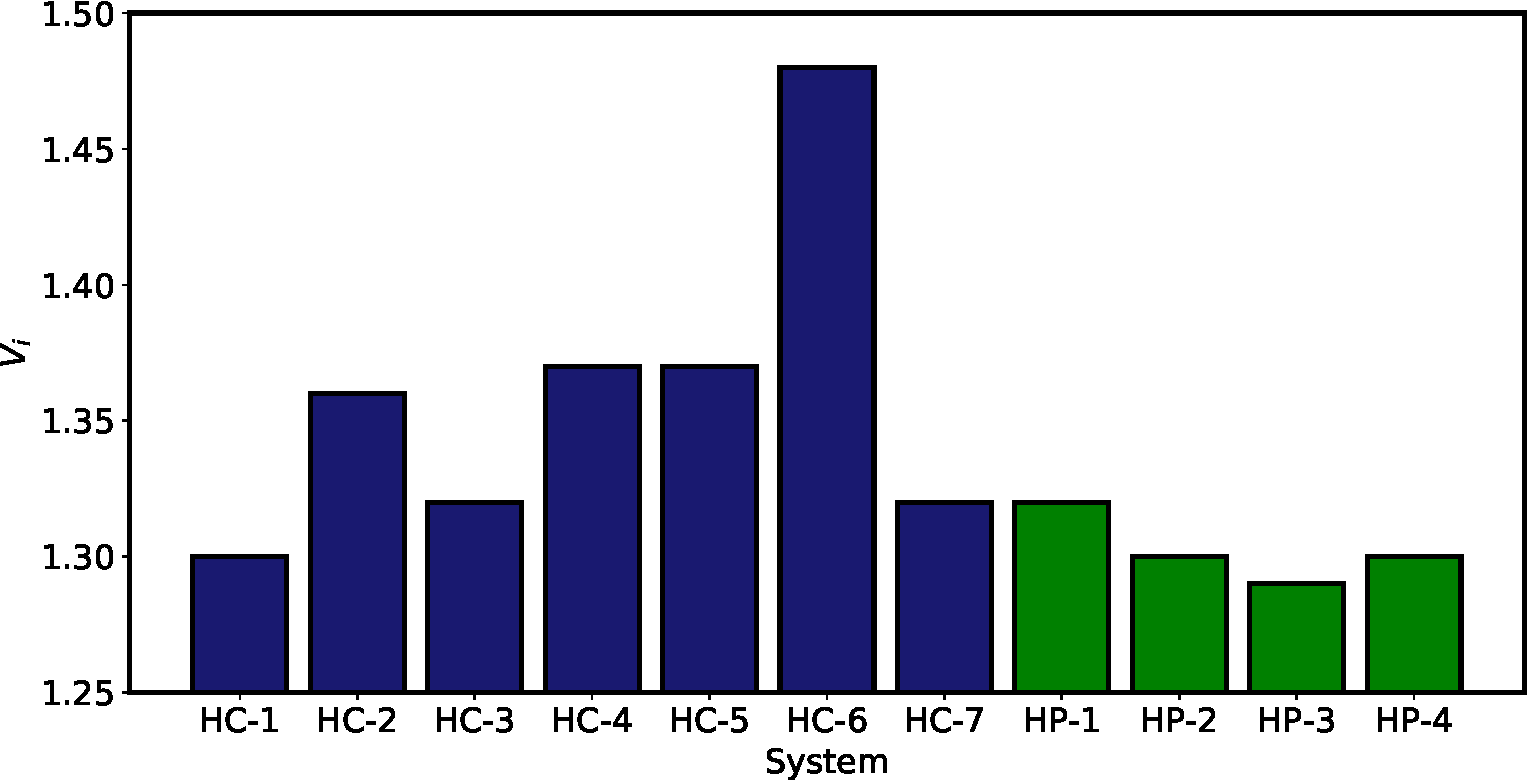
\includegraphics[width=0.8\linewidth]{Voronoi_Index}
  \caption{Voronoi indices for \textbf{HC} and \textbf{HP} crystal structures.}
  \label{figure: voronoi_index}
\end{figure}

We begin by analysing the crystal structures of the eleven compounds (\ref{table: chalcones}). The crystalline environment of each crystal can be examined initially from the perspective of a monomeric chromophore. To this end, we use Voronoi cell volumes $V_{cell}$ and van der Waals volumes $V_{vdW}$ to determine a Voronoi index $V_{i}=V_{cell}/V_{vdW}$, a metric for the spatial environment for a monomer in the crystal. $V_{i}$ values (Figure \label{figure: voronoi_index})  range from 1.29-1.48, showing that despite the substituent and packing differences, the  normalised spatial volume is comparable for all systems under investigation.  The $V_{i}$ values are such that there is little difference between the systems in terms of accessible volume for each chromophore when encapsulated by its neighbouring molecules.

To further deconstruct the intermolecular relationships, we examine the topology of the molecular crystals of \textbf{HC} and \textbf{HP} families by considering dimer packing motifs. Exciton transport has been shown to occur through coherent or incoherent hopping between molecular sites, and thus it is important to understand the possible intermolecular transport channels in the \textbf{HC} and \textbf{HP} systems.

\begin{figure}
\centering
  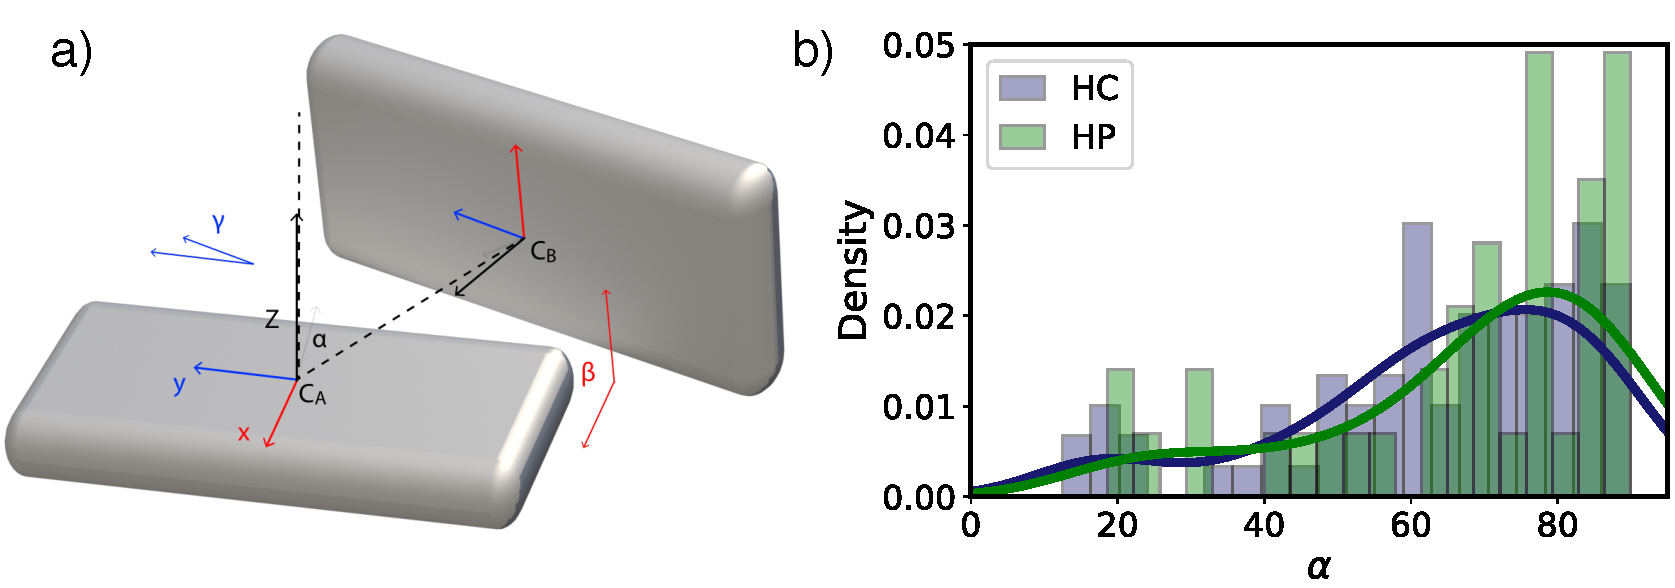
\includegraphics[width=0.8\linewidth]{dimer_schematic_alpha}
  \caption[Schematic of $\alpha$, $\beta$, and $\gamma$ angles for classification of dimers.]{Panel a), left; schematic of two monomers A and B, their centroids $C$, and the $\alpha$, $\beta$, and $\gamma$ angles used to classify dimer configurations. Panel b), right; distribution of $\alpha$ angles for dimers in \textbf{HC} and \textbf{HP} systems.}
  \label{figure: dimer_schematic_alpha}
\end{figure}

\begin{figure}[H]
\centering
  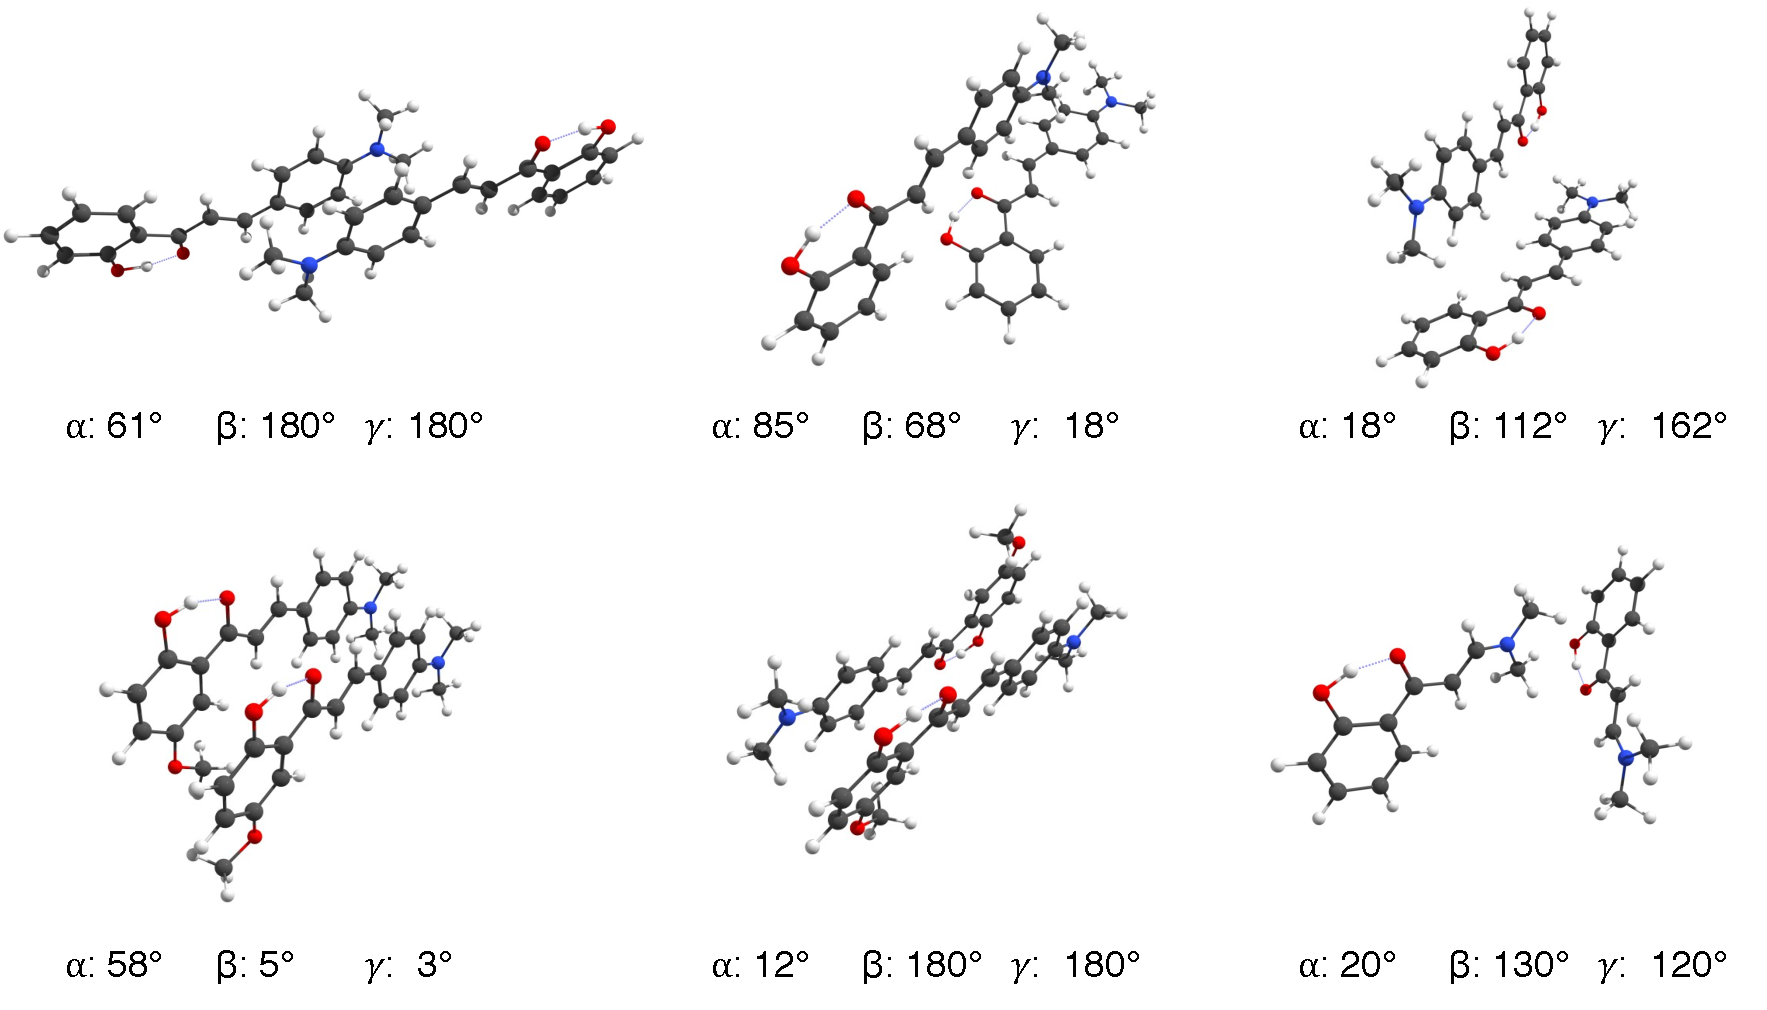
\includegraphics[width=0.8\linewidth]{motif_examples}
  \caption[Example dimer motifs in \textbf{HC1}, \textbf{HC5}, and \textbf{HP1}.]{Example dimer motifs and associated $\alpha$, $\beta$ and $\gamma$ angles in \textbf{HC1}, \textbf{HC5}, and \textbf{HP1}.}
  \label{figure: motif_examples}
\end{figure}

The dimer motifs are quantified through three angle variables, $\alpha$, $\beta$, and $\gamma$. These are depicted in Figure \ref{figure: dimer_schematic_alpha}, and example motifs with associated angles are given in Figure \ref{figure: motif_examples}. Three axes, $x$, $y$, $z$, are defined on each molecule A and B of the dimer, where $x$ and $y$ are the short and long axes of the molecule, and $z$ is the orthogonal unit vector. The angles are then defined as:
\begin{itemize}
\item[$\bullet$] $\alpha$: The angle between the $z$-axis located at $C_{A}$ and the vector connecting the two centroids $C_{A}$ and $C_{B}$.  The $\alpha$ angle quantifies the spatial overlap between the two monomers, ranging from 0\degree{} to 90\degree{}. 

\item[$\bullet$] $\beta$: The angle between the two short axes $x$ of each molecule, ranging from 0\degree{} to 180\degree{}, tracking whether monomers are aligned cofacially parallel ($\beta=$0\degree{}, CoF-P), or cofacially antiparallel ($\beta=$180\degree{}, CoF-A), or in a herringbone edge-face manner (90\degree{}, Hb), and all configurations in between. $\beta$ is thus often described as the ``herringbone'' angle. 

\item[$\bullet$] $\gamma$: The angle between the long-axis vectors $y$, ranging from 0\degree{} (parallel, P) to 180\degree{} (antiparallel, A). At $y=$ 90\degree{}, the dimer is T- or L-shaped, dependent on the $y$-slip. 
\end{itemize}

In Figure \ref{figure: dimer_schematic_alpha}b the distribution density of the $\alpha$ angle is shown for the \textbf{HC} and \textbf{HP} systems. The distribution is heavily skewed towards 90\degree, indicating that for the majority of dimers, there is little overlap between the centroids of the monomers. This is also apparent in Figure \ref{figure: yslip_density}, where the distribution of $y$-slip distances is shown. As such, it can be expected that in each molecular crystal there are few dimers with the classical configuration expected for efficient charge or energy transfer. This links back to the findings of Martinez and Iverson, in Section \ref{section: lom introduction}, who found a paucity of dimers with direct facial stacking.\cite{Martinez2012}

\begin{figure}[H]
\centering
  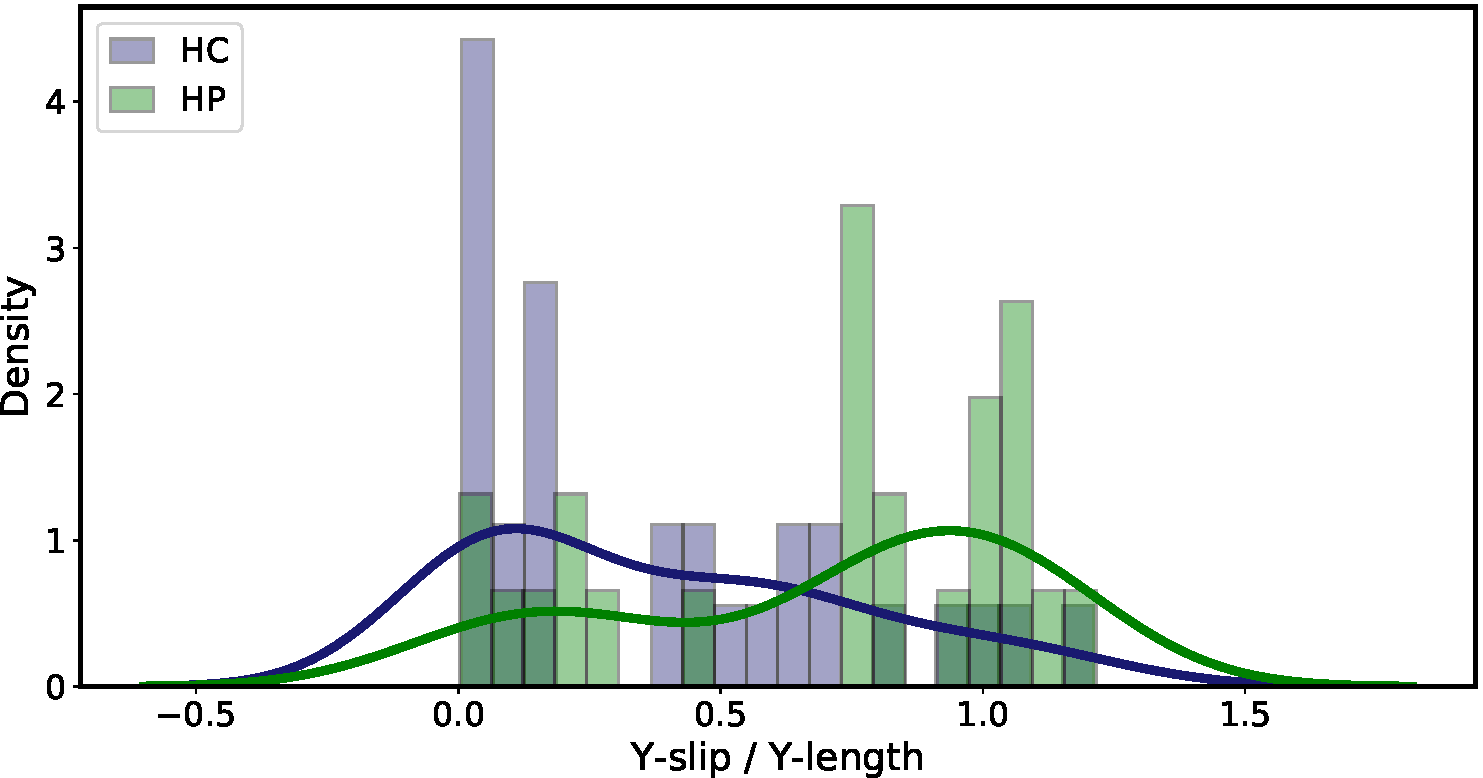
\includegraphics[width=0.8\linewidth]{yslip_density}
  \caption{$y$-slip densities for dimer configurations of \textbf{HC} and \textbf{HP} systems}{The density of slip distances for each molecular dimer in the $y$-plane (long axis). $Y$-length represents the length of molecule, such that the slip distance reported is independent of the chromophore identity.}
  \label{figure: yslip_density}
\end{figure}

Figure \ref{figure: dimer_classification} shows the dimer distribution densities for the $\beta$ and $\gamma$ angles for \textbf{HC} (top row) and \textbf{HP} (bottom row). Key regions are highlighted as an example in the upper plot of panel a); for example at $\beta$=90,$\gamma$=0, a herringbone (Hb) stack is witnessed with the long axes arranged in parallel. For both \textbf{HC} and \textbf{HP} systems, the majority of dimers have $\beta$ and $\gamma$ angles close to 180\degree{} (top right of plot), indicating that the most common dimer configuration is a cofacial arrangement where the carbonyl groups align antiparallel, at opposing ends of the molecule from eachother. This results in an antiparallel alignment of the \sone{} transition dipole moment of each monomer.  However, as panels b) and c) show, when the $\alpha$ angle is used as a filter, these cofacial arrangements occur at large slip displacements in the $x$ or $y$  plane ($\alpha$\textgreater{60}), and thus are more like edge-edge coplanar arrangements rather than the well-known $\pi$-stack. Only in \textbf{HC-5} is there significant cofacial $\pi$-stacking between dimers, with other cofacial arrangements in \textbf{HC} and \textbf{HP} having larger $y$-slip, as is common  for aromatic motifs. For \textbf{HC} compounds, 63\% of the cofacially aligned dimers have a $y$-slip of less than half a molecule, whereas 68\% of cofacially-algined \textbf{HP} dimers have a $y$-slip of more than half a molecule (Figure \ref{figure: yslip_density}), indicating the cofacial, $\pi$-stacked alignment is more prominent in \textbf{HC} compounds than their mono-aryl \textbf{HP} counterparts. 

\begin{figure}
\centering
  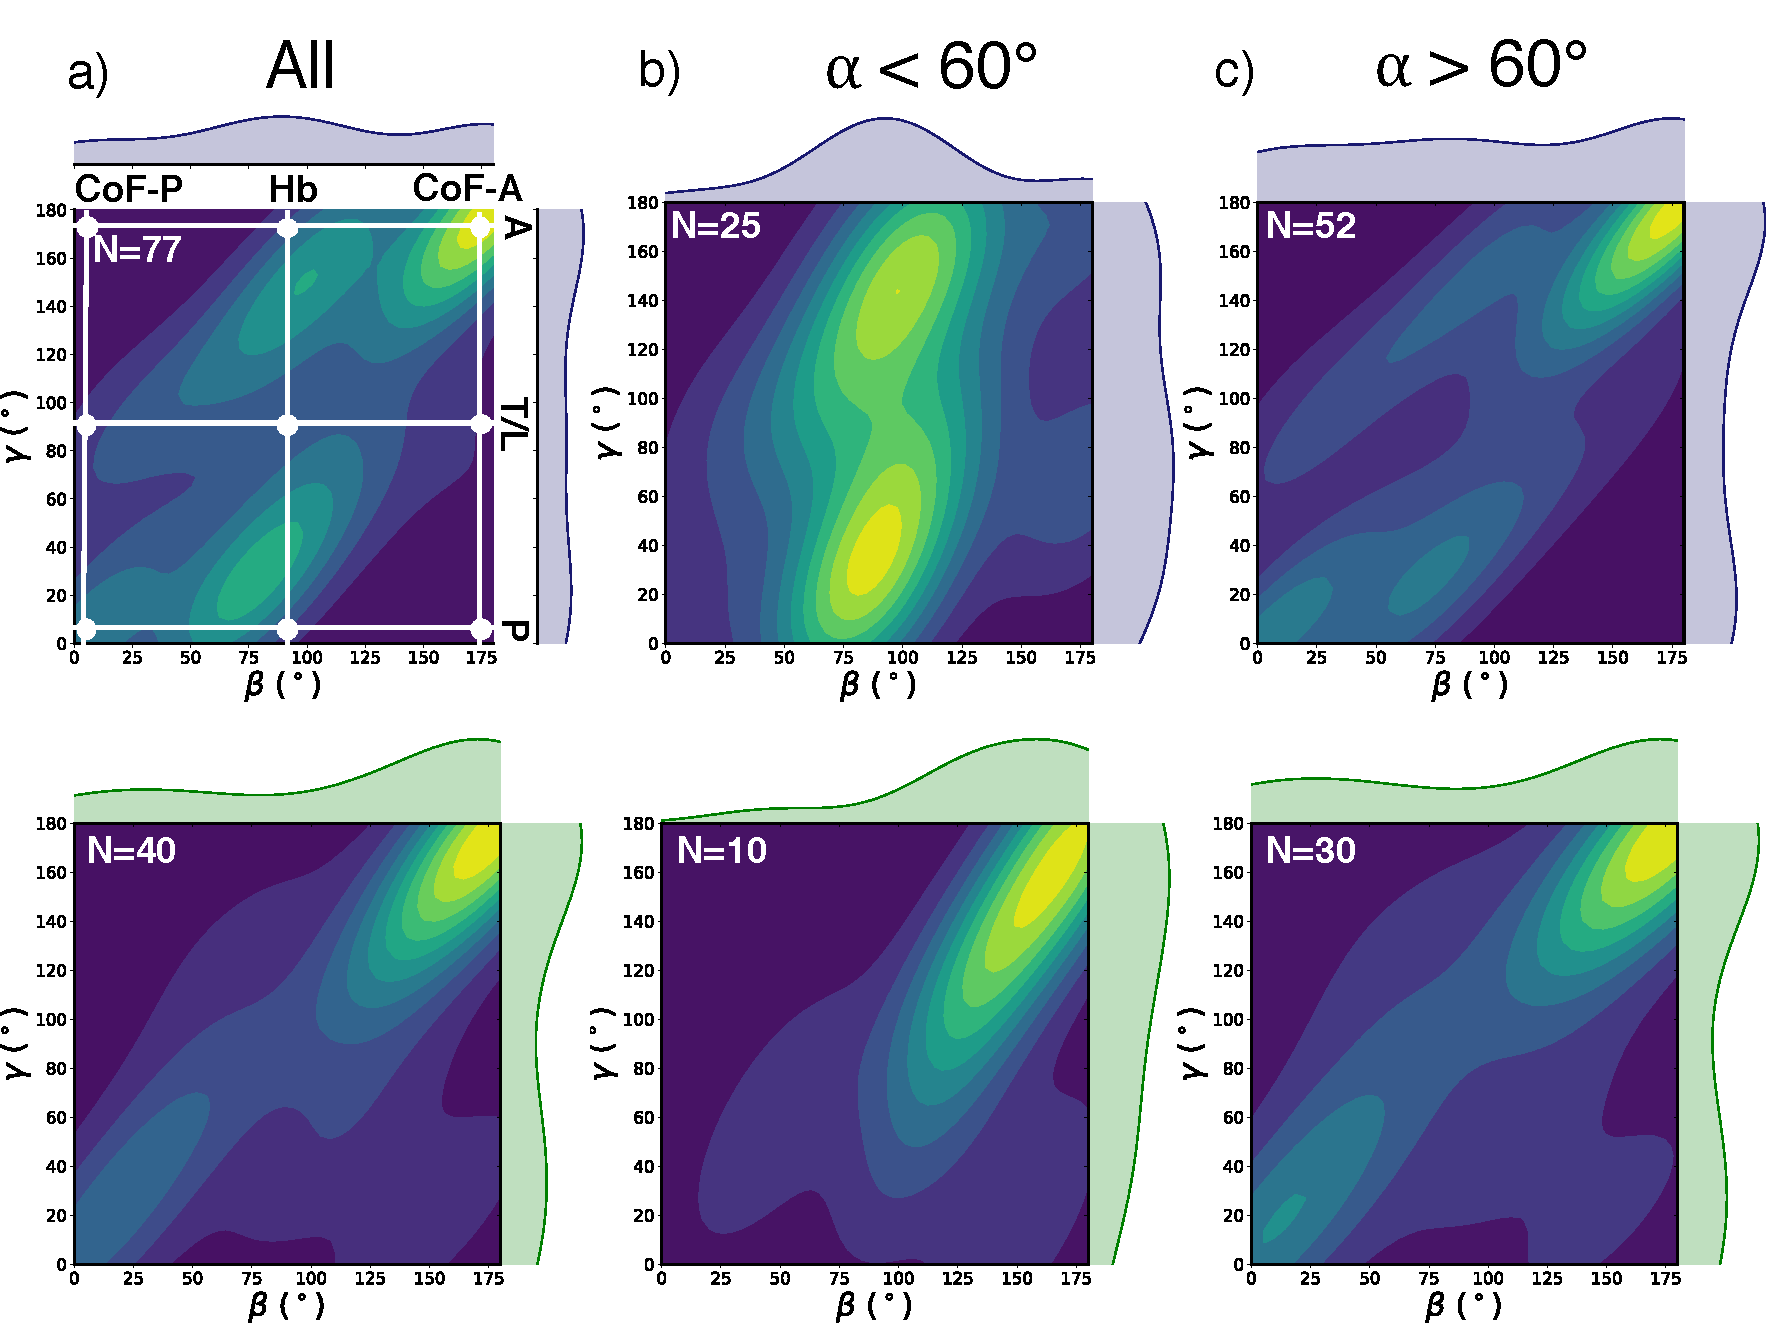
\includegraphics[width=0.8\linewidth]{dimer_classification}
  \caption[Probability density maps of $\beta$ and $\gamma$ angles.]{Panel a), left; Probability density map of the $\beta$ and $\gamma$ angles for \textbf{HC} (top) and \textbf{HP} (bottom) dimers. Key configurations are labelled on the axes, as explained in the text. Panel b), centre; probability density for the subset of dimers where $\alpha$ \textless{}  60\degree{}.  Panel c), right; probability density for the subset of dimers where $\alpha$ \textgreater{} 60\degree{}.}
  \label{figure: dimer_classification}
\end{figure}

For the dimers with significant overlap (Figure \ref{figure: dimer_classification}b), \textbf{HC} has two hotspot regions with $\beta$ approximately 90\degree, indicating a herringbone arrangement, with carbonyl groups at the same ($\gamma=$0\degree) or opposite ends of the dimer ($\gamma=180\degree$). There also exist dimers close to this arrangement, with deviations in both $x$ and $y$. Conversely, in the relatively few \textbf{HP} systems with  $\alpha$\textless{60}, configurations lie on the diagonal, indicating motifs centred around a T-shape, which move to L-shaped when $\alpha$\textgreater{60}. Overall, the significant dimer arrangement in \textbf{HP} compounds is a herringbone motif, with the majority of cofacial arrangements having a large $x$ or $y$-slip with minimal $\pi\pi$ interactions due to the single aryl groups aligning at $y$=180\degree. The $\alpha$ angle is generally larger than in \textbf{HC}, indicating a larger slip, with overlapping monomers distributed around a cofacial stacking. The prominence of the herringbone arrangement in \textbf{HC} systems is replaced by a propensity for a T-shape packing, quantified by the $\gamma$ angles distributed around 90\degree. In the next section, we show how these geometric parameters, and those of the chromophore, influence the exciton coupling in the \textbf{HC} and \textbf{HP} families.
\subsection{Intermolecular interactions in the molecular crystal}\label{section: Connecting_Interactions}

Localisation of the electronic excited state onto one monomer of the molecular crystal has been shown to be an important step in the relaxation process of ESIPT systems in the solid state. For the dimers discussed above, the coupling $J_{ij}$ between monomers $i$ and $j$ is calculated in Troisi's diabatization scheme based on the orthogonal transformation of adiabatic states to diabatic states (Equation \ref{equation: diabatic matrix}).\cite{Arago2015,Fornari2016}. In this Chapter this method is extended to asses the effect of a third monomer $k$ on the exciton coupling, where in a trimer chromophore, $\textbf{H}^D$ becomes a 3x3 matrix
\begin{equation}
\small
\label{equation: 3x3 diabatic matrix}
\begin{bmatrix}
E_{i}^D & J_{ij} & J_{ik}\\
J_{ji} & E_{j}^D & J_{jk} \\
J_{ki} & J_{kj}& E_{k}^D
\end{bmatrix}
=
\begin{bmatrix}
C_{11} & C_{12} & C_{13}\\
C_{21} & C_{22} & C_{23}\\
C_{31} & C_{32} & C_{33}
\end{bmatrix}
\begin{bmatrix}
E_{i}^A & 0 & 0\\
0 & E_{j}^A & 0\\
0 & 0 & E_{k}^A\\
\end{bmatrix}
\begin{bmatrix}
C_{11} & C_{12} & C_{13}\\
C_{21} & C_{22} & C_{23}\\
C_{31} & C_{32} & C_{33}
\end{bmatrix}
\end{equation} 
where the coupling $J_{ij}$ between monomers $i$ and $j$ incorporates the effect of monomer $k$, which can quantified through comparison of the dimeric and trimeric $J_{ij}$. Analysis of excitations at the Franck-Condon geometry for a trimer chromophore show that for \textbf{HP1}, the bright state is delocalised over two of the molecules arranged in a cofacial arrangement. This is shown in Figure \ref{figure: trimer_excitations}. A delocalised state over the whole trimer is not observed. Analysis of the excitations of the three types of dimer inherent in the trimer reveal that in each case, regardless of the stacking arrangement, the excitation is delocalised over both monomers. 

\begin{figure}[H]
\centering
  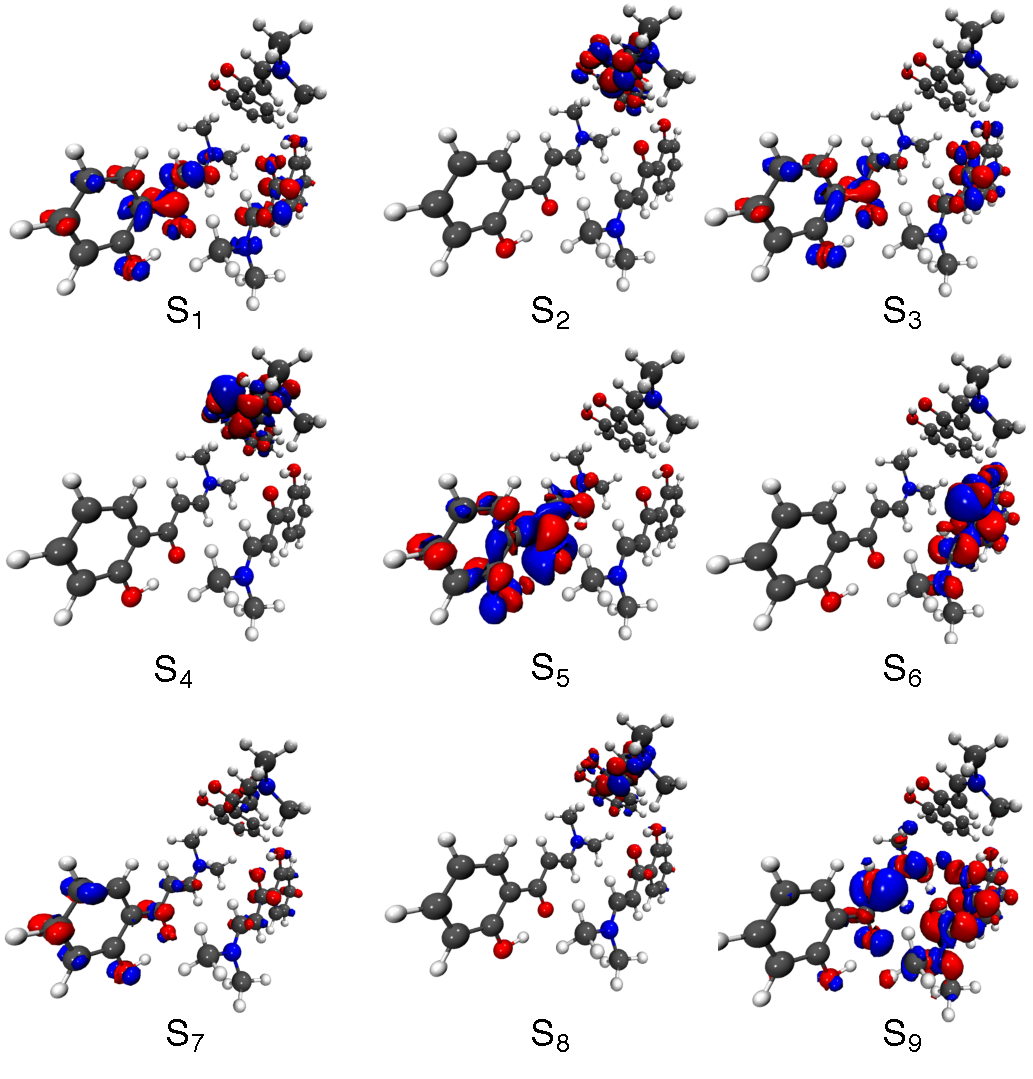
\includegraphics[width=\linewidth]{trimer_excitations}
  \caption[Electron density diffrence maps for the first nine excited state of the \textbf{HP1} trimer.]{Electron density diffrence maps for the first nine excited state of the \textbf{HP1} trimer. The same colour scheme is used as in Figure \ref{figure: HC_Vac_Densities}}
  \label{figure: trimer_excitations}
\end{figure} 


With this in mind, we  calculated the dimer exciton coupling for a trimer system to assess the impact of an exterior monomer on the dimer coupling in \textbf{HP1}, \textbf{HC1}, and \textbf{HC5}. It is found that the addition of a third molecule has only a small effect on the dimer coupling in \textbf{HP1} and \textbf{HC1}, where the increased coupling in one dimer is compensated for by the decreased coupling in the other dimer, with difference of less that 0.02 eV. The largest effect is seen in \textbf{HC-5} due to the cofacial packing of the trimer system, where the central monomer is sandwiched by two cofacially stacked monomers, one parallel and one antiparallel.  These purturbations are no larger than the inherent modulation of couplings in the dynamic regime.\cite{Arago2015,Arago2016} As such, focus from here will be on dimer couplings where the presence of exterior molecules has been neglected. The exciton couplings and the identity of the dimer with the largest $J$ are shown in Figure \ref{figure: couplings}.

\begin{figure}
\centering
  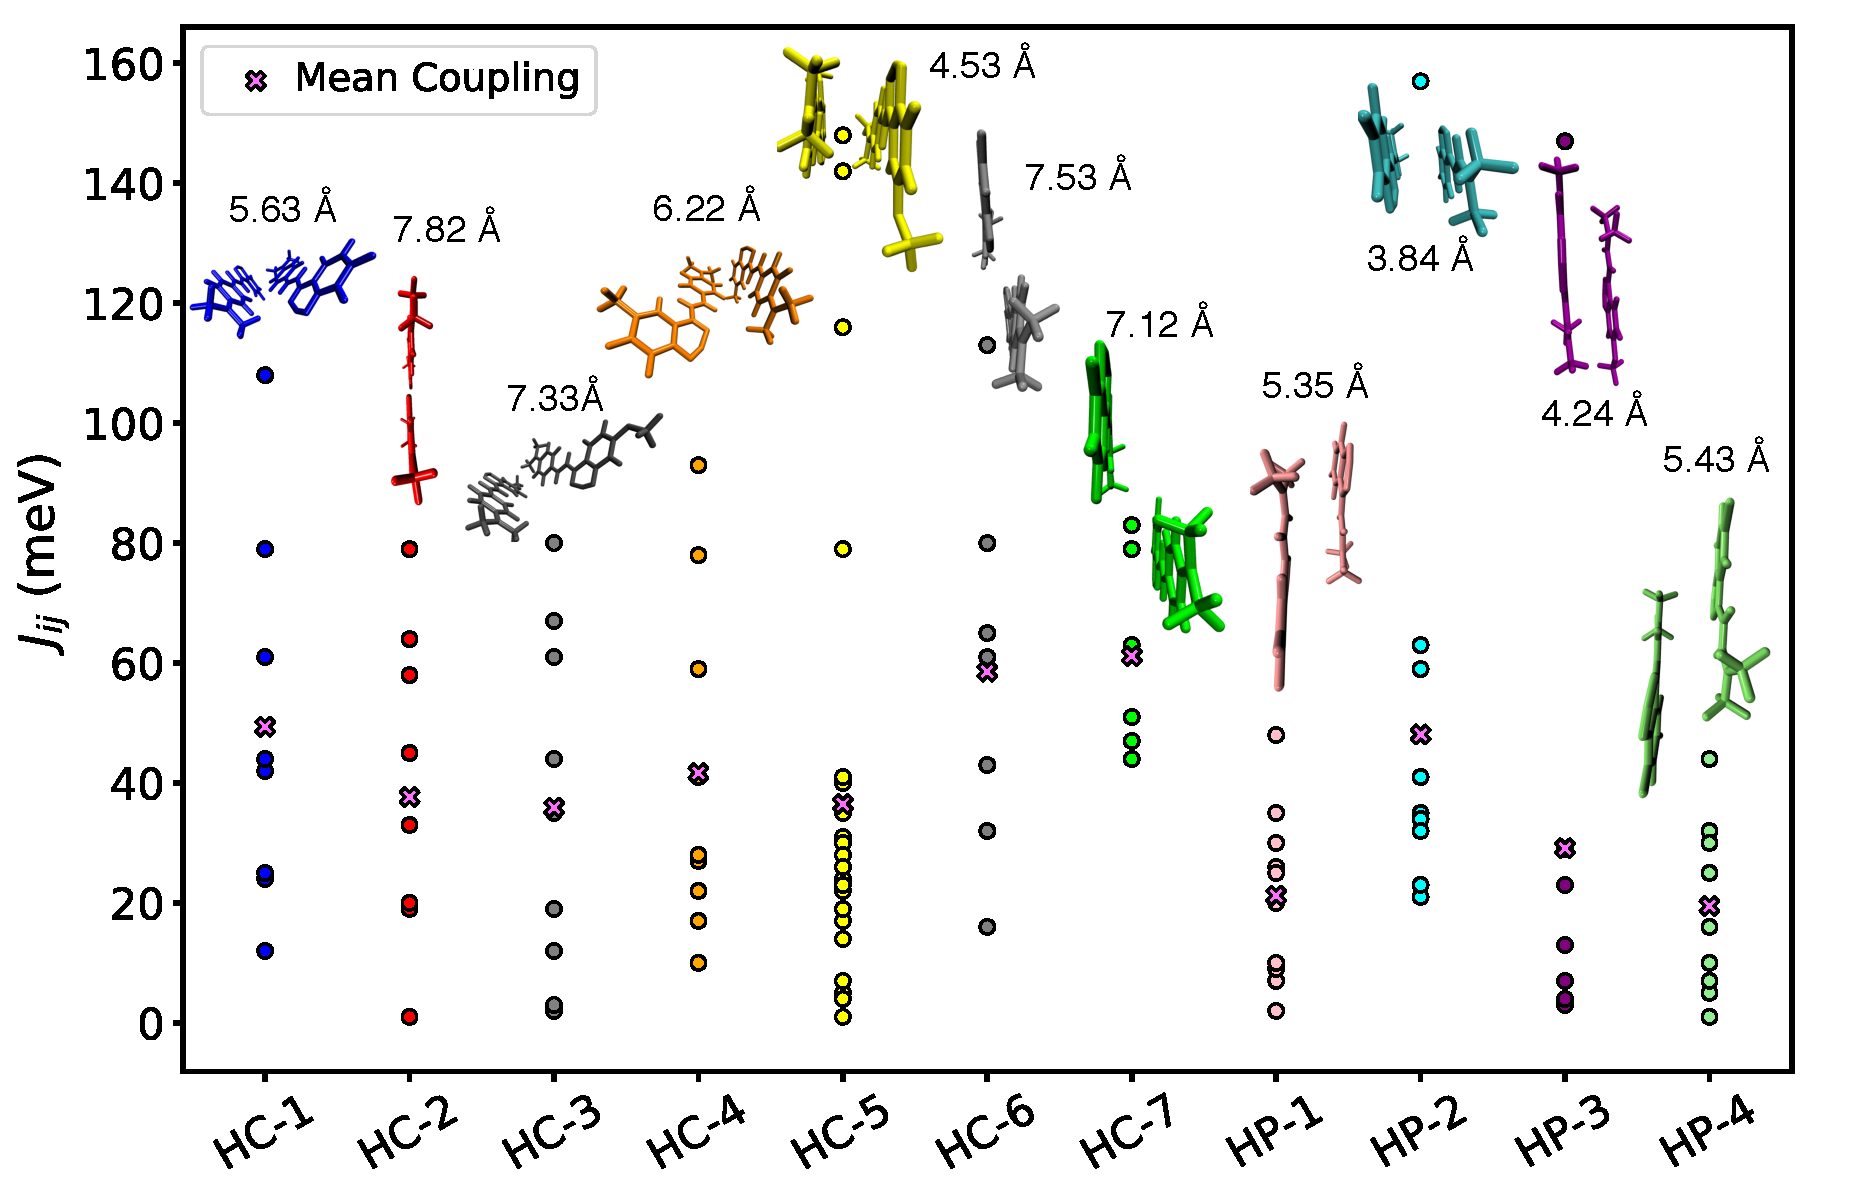
\includegraphics[width=0.8\linewidth]{couplings}
  \caption[Exciton couplings in \textbf{HC} and \textbf{HP} systems]{Exciton couplings $J$ between monomers $i$ and $j$ in the dimers identified in \textbf{HC} and \textbf{HP}. The mean coupling is also shown, along with the distance in angstroms between the constituent monomer centroids.}
  \label{figure: couplings}
\end{figure}

In \textbf{HC1-4}, where the closest packed dimers are herringbone in nature, similar dimer configurations are present. For \textbf{HC-2}, the identity of the dimer with the largest coupling changes due to a lateral displacement of one monomer increasing the centroid distance to 8.5 {\AA} and thus reducing the coupling in the herringbone stacked dimer. The identity of the largest coupled dimer changes to a cofacial, edge-edge stacked dimer with $\alpha=87\degree$, where minimal overlap reduces the coupling $J$. For \textbf{HC-1,3,4}, the herringbone stacking pattern is exhibited where the largest coupling is found in \textbf{HC1}, where the monomers are most tightly packed. In \textbf{HC5-7}, face-face stacked dimers are more prevalent in the crystal structure. The size of the coupling in \textbf{HC6} is reduced compared to \textbf{HC5} due to the $x$ displacement of one the monomers. It is further reduced in \textbf{HC7} due to an increased $y$-slip. In the \textbf{HP} compounds, the large $\alpha$ and $y$-slip values systematically reduce the average coupling. In each \textbf{HP} derivative there exists one close packed, cofacial dimer which exhibits the largest coupling. In \textbf{HC2-3}, the crystal structures afford more efficient cofacial stacking with y-slip values of only 1{\AA}, resulting in the largest couplings of all investigated systems. 

As shown in  Figure \ref{figure: dimer_regressions}a, the coupling $J$ correlates linearly with half of the energy splitting for the \sone{} and \stwo{} states of the dimer. This is somewhat surprising, given the simplicity of the original model (Section \ref{section: lom intermolecular-interactions}), the polarity of the molecules in question and their generally nonparallel stacking. The energy splitting is perhaps the simplest way to obtain the exciton coupling in the Kasha regime, although it is more expensive than using atomic-centred transition charges, or the PDA approximation, since the supramolecular calculation must be done rather than one monomer calculation. At small intermolecular distances (\textless4{\AA}), these computationally efficient metrics can underestimate the couplings due to them only considering the Coulomb interaction.\cite{Kistler2013} The linear correlation here shows that the general Kasha interpretation of the coupling applies here and that the diabatization method to obtain the couplings reproduces the supramolecular coupling.

We investigate the role of H- and J-aggregates by assigning dimers based on the oscillator strength of the \sone{} (J) and \stwo{} (H) excitation, which offers better resolution than using the energy shift. This is summarised in Table \ref{table: dimer_types}.  In \textbf{HC}, systems, 60\% of dimers are J-aggregates, while in \textbf{HP} systems the J-aggregate population is 58\%. For \textbf{HC-4} and \textbf{HC-5}, which are nonemissive, the J-aggregate population drops to 22\% and 32\%, respectively. Important to note, however, is that emission in K* is from a localised excited state, and thus monomer regime should dominate the emission characteristics. In ESIPT systems, the role of H- and J-agggregates is expected to be prominent only at absorption, and the J-aggregates are not responsible for the AIE behaviour due to the localised emission.

\begin{table}
\caption[Dimer types for \textbf{HC} and \textbf{HP} molecular crystals]{Dimer types located for each molecular crystal. Significant increase in \textbf{HC5} dimers due to rotational flexibility of the methoxy group} 
  \label{table: dimer_types}
  \begin{tabular}{cccc}
  \hline
  System & H-aggregates & J-aggregates & Total\\
  \hline
  \textbf{HC1} & 4 & 4 & 8\\
  \textbf{HC2} & 5 & 4 & 9 \\
  \textbf{HC3} & 4 & 5 & 9\\
  \textbf{HC4} & 7 & 2 & 9\\
  \textbf{HC5} & 19 & 10 & 29 \\
  \textbf{HC6} & 4 & 3 & 7\\
  \textbf{HC7} & 6 & 0 & 6\\
  \hline
  \textbf{HP1} & 5 & 5 & 10\\
  \textbf{HP2} & 5 & 6 & 11\\
  \textbf{HP3} & 4 & 5 & 9\\
  \textbf{HP4} & 5 & 5 & 10\\
  \hline
  \end{tabular}
\end{table}

In the Kasha model, for a perfectly stacked dimer with no $y$-slip, the oscillator strength of the \stwo{} state should be double that of the monomer state. Figure \ref{figure: dimer_regressions}b shows the relationship between the $y$-slip in the dimers and the oscillator strengths of the \sone{} and \stwo{} states. This trend is apparent in these systems, where the y-intercept of the model for \textbf{HC} is 2.26, with the average oscillator strength is 1.16. For \textbf{HP} systems the mean monomer oscillator strength is 0.53, with the model predicting the dimer osillator strength as 0.95. With increasing $y$-slip, the difference in oscillator strength between the two states also decreases until the inversion to J-aggregates is witnessed ($f_{S_{1}}>f_{S_{2}}$). The largest group of outliers are cofacially stacked dimers, where a larger shift is seen at lower slip distances due to the minimal $x$-slip and archetypal stacking.\cite{Gierschner2016} 

